\chapter{Systeemarchitectuur}
\label{chap:architectuur}

\section{Model}
\label{sec:model}
CalZone is een webapplicatie. Gebruikers van het systeem bezoeken de applicatie via hun webbrowser. Deze browser kan de browser op hun computer zijn of op de Android browser op hun smartphone.
\\
CalZone heeft als architectuur gekozen voor het MVC-patroon.\cite{mvc}

\begin{figure}[H]
	\centering
	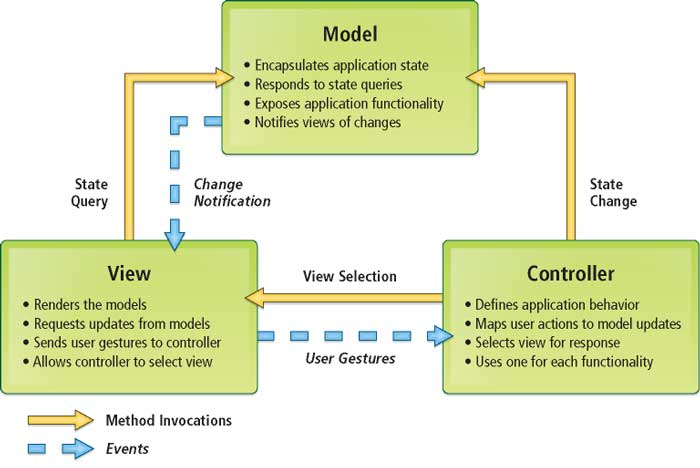
\includegraphics[scale=0.5]{img/mvc}
	\label{fig:mvc}
	\caption{Een voorstelling van de werking van een systeem gebruikmakende van een MVC architectuur}
\end{figure}

\section{Gebruikte technologie}
\label{sec:technologie}
De programmeertaal die gebruikt wordt, is Java. 
In Java wordt gebruik gemaakt van het Spring MVC framework\cite{spring, spring-mvc} voor het ontwikkelen van CalZone. 
De IDE waarin geprogrammeerd wordt, is de meest recente versie van 'Eclipse Classic' met volgende uitbreidingen:

\begin{itemize}
	\item De gehele collectie 'Web, XML, Java EE and OSGi Enterprise Development'	
	\item Spring Tool Suite (uit de Eclipse Marketplace)
	\item De gehele collectie 'Maven Integration for Eclipse'
\end{itemize}
\noindent
Het uitvoeren van de applicatie wordt mogelijk gemaakt door middel van Apache Maven\cite{Maven} en Apache Tomcat\cite{Tomcat}.
De gebruikte databank voor de back-end is MySQL. 
Voor de view wordt gebruik gemaakt van JSP's: een tehnologie om dynamisch webpagina's te genereren.
